
\section{Transformer and Attention}

The Transformer is a mechanism that is based entirely on attention. Strictly speaking this is not the attention explored in the Sequence to Sequence model in Chapter 1, though there are some similarities. It is a model that uses no recurrent components and no convolution components. 

Recurrent components have some negative qualities. Recurrent components are hard to run with batch input data. Also they do not work with very long data strings. 

If a batch of data is to be cycled through a recurrent component, we would like all that data to go through the component at the first cardinal position first. Then we would like it all cycled through the second or third position. In actuality the first time step the first part of the data needs to go through the first Recurrent Neural Network module and then the next component all the way to the last position in the model. Then the data can be moved along to the second time step where the Recurrent Neural Network module sees the second part of the data which is processed through all components of the GRU. At some point the third part of the data is seen, and all data after that is processed the same way.

Also because the Recurrent Neural Network is so heavy with Neural Network components, many weights and biases, though they can remember patterns, they loose some information with every pass. This is why there is a practical limit to the length of the input sequences that the typical Recurrent Neural Network can use. This is why the length of sentences in network models that use the Recurrent Neural Network are short.

Transformers use no Recurrent Neural Network components. Their operations can be parallelized so that large batches of data can be processed at once during the same time step. 

Longer sequences can be considered as well, so Transformer input can contain longer English language sentences and even paragraphs.

\subsection*{Byte Pair Encoding}

\ac{BPE} stands for `Byte Pair Encoding.' WordPiece is a particular implementation of Byte Pair Encoding.

WordPiece is used by some transformer systems to encode words much the way that Word2Vec does. Like Word2Vec, WordPiece  has a vocabulary list and a table of embeddings that maps one word or token to a vector of a given size.

WordPiece, though, handles Out Of Vocabulary (OOV) words gracefully. It breaks large words into smaller pieces that are in the vocabulary, and has a special notation so that these parts can easily be recombined in order to create the input word again. Byte Pair Encoding is not so interested in pre-trained word embeddings like Word2Vec and Glove.

For the Generative Pre-training Transformer 2 a version of Byte Pair Encoding is used instead of a vocabulary system like Word2Vec or Glove.

Some form of Byte Pair Encoding is included in almost every Transformer typed Neural Network model, so no decision needs to be made about what type of word embeddings to use.

\subsection*{Attention}
Attention mechanisms are used in a similar way in three places in the model. The first implementation of the Self Attention is discussed below.

It should be noted that input to the Transformer is strings of words from a desired input language. Output is similarly words in a given language. Input words are treated very much the way that they are in Sequence to Sequence models. A word is translated to a number and that number indexes an entry in a word-to-vector table. From that time forward a word is represented by a vector of floating point numbers. In a transformer this word vector can be large. In the original paper Vaswani et al (2017)\cite{Vaswani2017AttentionIA} use a vector size of 512. 

\subsection*{Scaled Dot-Product Attention}

The Transformer has a signature self-attention mechanism. This is possibly one third of the entire Transformer mechanism, but a variety shows up in the other two-thirds. 

The first thing that happens is the input word vector is converted to three other values. These new vectors are like the input vector but they have a smaller dimensionality. Converting the word vector in this way is accomplished by three simple matrix multiplication operations.

In the diagram below a simple conversion of this type is illustrated. In the diagram we convert a vector with dimension of 1x3 to a dimension of 1x2. In reality we are converting a vector from 1x512 to 1x64. This is a division of 8.



\begin{figure}[H]
	\begin{center}
		
	
	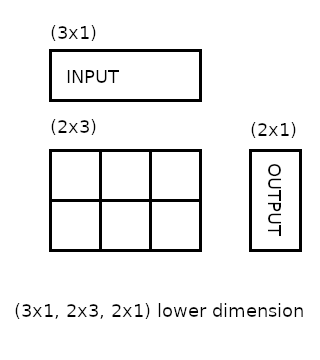
\includegraphics[scale=0.5]{diagram-mat01}
\end{center}
	\caption[Lowering Dimensionality]{Lowering Dimensionality}
	
	%\addcontentsline{lof}{section}{Loss and Accuracy}
\end{figure}


One thing we want to do is to preserve the dimension of our vector. We start with a 512 sized floating point vector and after some processing we want to return to the same size. Before that is done the vector is processed at the smaller size of 64. 

In this self-attention scheme three vectors are actually required. All three vectors are sized 64, and all three are converted by separate matrix multiplication operations. The weights to convert each of the three vectors are different. For this reason the new smaller vectors are all different.

The smaller vectors individually are called q, k, and v. They can also be referred to as larger matrices. The new vector matrices are denoted as Q, K, and V. Q stands for `Query'. K stands for `Key'. V stands for `Value'. 

The Query value is multiplied by the Key values from all vectors in the input. This multiplication is `dot-product' multiplication. When it is done all keys will have low output except those that are closest to the Query. Then the results are passed through a softmax function. When this is complete there will be a single vector that is close to 1 and another group of vectors that are all close to 0.

The vector produced by multiplying the softmax with the V values of every word produces a single word vector that is close to its original value, and many others that are near zero.

This formula from Vaswani et al (2017)\cite{Vaswani2017AttentionIA} 
shows the process.

$$
\mathlarger{ \mathlarger{
Attention(Q,K,V)=softmax(\dfrac{QK^T}{\sqrt{d_k}})V
} }
$$

Here the value of $\sqrt{d_k}$ is used to limit the size of the $QK^T$ output and $d_k$ is the dimension 512. Without this the softmax function has to deal with much larger numbers. Smaller numbers for the softmax are preferred. 

The function can actually perform this on large matrices with high dimensionality, in parallel. This parallel matrix operation increases the speed of training.

In the green triangle in the Figure 2.2 we preform the multiplication and selection that was just described.

\begin{figure}[H]
	\begin{center}
		
		
		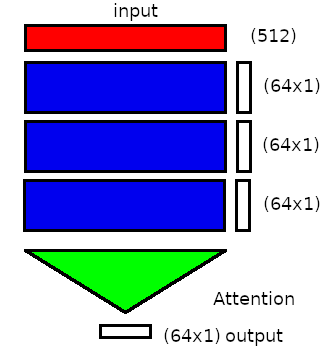
\includegraphics[scale=0.5]{diagram-mat03-64}
	\end{center}
	\caption[Attention Output]{Attention Output}
	
	%\addcontentsline{lof}{section}{Loss and Accuracy}
\end{figure}




Finally the output we calculated above must be returned somehow to the input dimensionality. This is accomplished by duplicating the procedure described eight times with eight separate weights. When this is done the output of the attention mechanism is concatinated together, returning the output to the proper size.

This multi-headed approach allows different heads to learn different types of relationships, and then when they are grouped together the learned relations are recovered and contribute to the output.

\begin{figure}[H]
	\begin{center}
		
	
	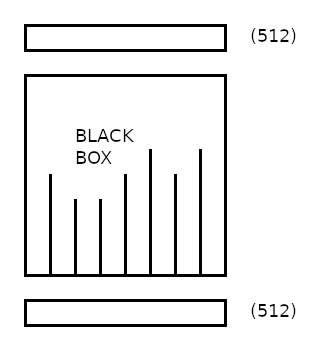
\includegraphics[scale=0.5]{diagram-mat02}
\end{center}
	\caption[Matching Input and Output]{Matching Input and Output}
	
	%\addcontentsline{lof}{section}{Loss and Accuracy}
\end{figure}


Later the output is passed through a feed forward network. After that it is combined with the original input again through addition. Then the vectors are normalized. This makes sure that the values are all within reasonable ranges.

This describes the encoder section. There are two other attention segments. Together these two sections combine to form the decoder section.

\subsection*{Transformer - Decoder}
The decoder is composed of two attention mechanisms and a feed-forward segment. The result of the encoder's work is passed to the decoder and remains applied to one of the decoder's attention mechanisms throughout the decoder's work. In that one of the two attention mechanisms of the decoder the `Key' and `Value' matrices are imported from the encoder. 

While the encoder takes in the entire input and attends to whatever portion of that input it finds to be important, the decoder is interested in producing one token at a time. 

During inference it produces a token and then it adds to that token, one at a time, until the decoding is finished and something like a sentence is produced. It can attend to any part of the output it has already produced. During training the decoder is exposed to the target sequence under a mask. The mask prohibits the decoder from seeing parts of the target that it should not. This mimics the inference setup and still allows for large input matrices.

We illustrated in the Sequence-to-sequence discussion the importance of the single `thought vector'. The Transformer can be seen as having a thought-vector also. There is a corridor of data from encoder to decoder. Two important smaller vector-sized inputs from the encoder are ultimately required in the decoder. They represent the `Key' and `Value' matrices. The matrices required are the size of the smaller, reduced, vector. The full sized vector is transported from the encoder and is reduced dimensionally in the decoder to two smaller matrices.

There is also a second attention mechanism in the decoder. It works solely on data from the decoder itself. It works very much like the attention mechanism from the encoder - only it attends to every word of output as opposed to the entire input sequence. It passes it's output to the layer described above. This data is lowered in dimensionality and becomes the `Query' matrix for that layer. During training this section is masked also.





\begin{figure}[H]
	\begin{center}
		
		
		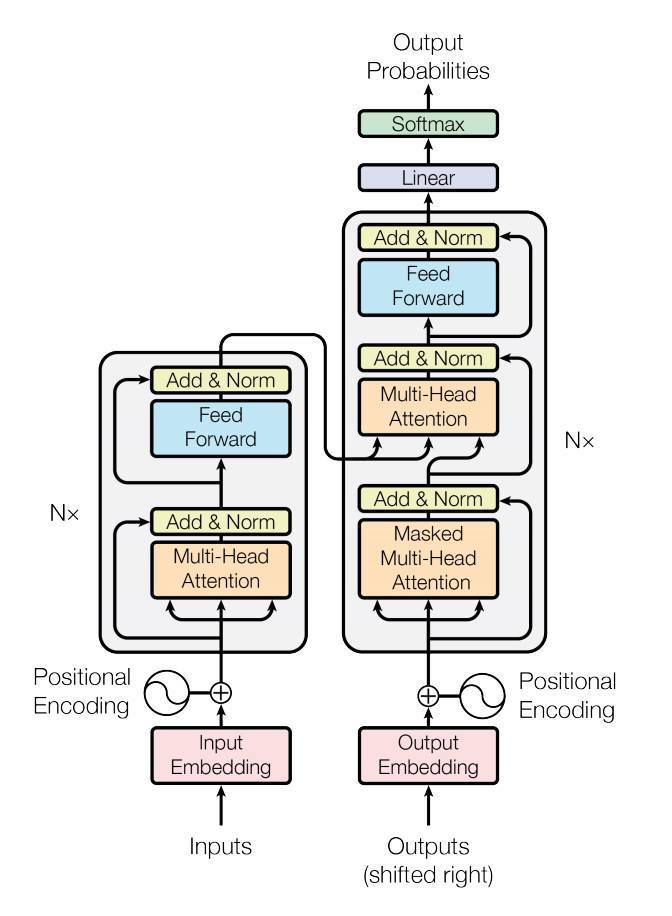
\includegraphics[scale=2.0]{diagram-mat04}
	\end{center}
	\caption[Transformer Encoder and Decoder]{Transformer Encoder and Decoder - Vaswani et al(2017)\cite{Vaswani2017AttentionIA}}
	
	%\addcontentsline{lof}{section}{Loss and Accuracy}
\end{figure}

\subsection*{Transformer - General}

The input of the Transformer encoder and decoder employ not only a word-vector table, but also a positional encoding scheme. The model adds to the input vector information that it can then use to learn the position of words in a sentence. 

Words that are early in the sentence have a certain appearance and words later on appear differently. The Encoder and Decoder use sine and cosine waves to impart this information onto the sentence sequence. 

Meanwhile at the output of the decoder the output vectors are processed through a linear matrix which increases the vector's dimensionality so that the output vector is the size of the output vocabulary dimensionality. After the linear matrix the vector is processed by a softmax function. Then the highest floating point value in the new larger vector is the index of the chosen output word.

The Transformer model takes large memory resources, large corpus resources, and large training time resources. Without these components the Transformer is not suitable for many projects.

\subsection*{Pre-Training}
Pre-Training is when the authors of a model train an instance and then make the model available to the public on-line. This is helpful for the average programmer interested in Neural Networks. Training an instance of the transformer model can use up computation resources for days, and require hardware that is costly. Usually the cost of producing a trained model is prohibitively expensive.

After acquiring a trained model, the programmer goes on to adjust the model to their task. Adjusting a pre-trained model to a given task is called `Transfer Learning'. Many tasks lend themselves to Transfer Learning. Conceptually a model can be fine-tuned to any problem and many problems can be addressed with good results after only modest fine-tuning.

There is a pre-trained Transformer model called \ac{BERT}. BERT stands for `Bidirectional Encoder Representations from Transformers'. The BERT files available on-line are mainly for classification tasks. They allow for input that uses a vocabulary size that is very large, but the output is meant to be smaller.

The `Bidirectional Encoder Representations from Transformer' models use a bidirectional training method. During training the BERT model might be presented with a sentence with a word missing. The training task is to fill in that blank. The model can look at the sentence from any direction in order to find that word. This is a very simplistic explanation for what is termed a Masked Language Model.

\subsection*{Visualization - Transformer}

In order to visualize what is happening during inference we have colorful charts that we can look at. In this chart we are looking at how each word attends to all the other words in the input text.

\begin{figure}[H]
	\begin{center}
		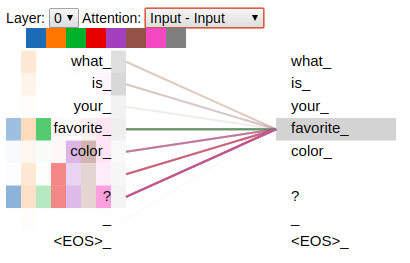
\includegraphics[scale=2]{Figure_3}
		
		
	\end{center}
	\caption[Visualized Attention]{Visualized Attention -- `favorite' shows attention to some but not all words in the sentence.}
	
	
\end{figure}

Significant is that words, like `what' and `your', do not have strong attention to words in the text on the right. In a chart like this one they would show no colors on the left and light colored lines connecting the left to the right.

This diagram is from the Transformer with the larger hyper-parameter set that we describe in Chapter 3, trained on the movie dialog corpus.

%Our model is not very large compared to the GPT2 model, and so it has not been trained on a corpus that has many Winograd-type examples. We speak about the Winograd schema at the end of the text.


\section{The Generative Pre-training Transformer 2 Model}

`Generative Pre-training Transformer 2' (\ac{GPT2}) is a large model. It is based on the Transformer from Vaswani et al (2017)\cite{Vaswani2017AttentionIA} but there are some major changes. The model uses the encoder portion of the Transformer without the decoder. There are some other changes to the output layers. The biggest difference is that it is pre-trained and downloadable.

It still uses Scaled Dot-Product Attention. A model diagram is taken from Radford et al (2018)\cite{radford2018improving}. A mask is used in the Self Attention segment of the model.

\begin{figure}[H]
	\begin{center}
		
		
		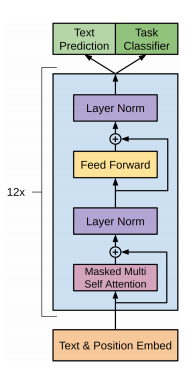
\includegraphics[scale=4.0]{diagram-mat05}
	\end{center}
	\caption[Generative Pre-training Transformer 2 ]{GPT2 - Radford et al(2018)\cite{radford2018improving}}
	
	%\addcontentsline{lof}{section}{Loss and Accuracy}
\end{figure}

There are several sizes of pre-trained `Generative Pre-training Transformer 2' model. They are all rather large. The smallest model matches the size of the largest `Bidirectional Encoder Representations from Transformers' model. The GPT2 models input and output text sequences. In this way they are preferred for our application over the BERT models. 

The `Generative Pre-training Transformer 2' models are trained on a corpus called WebText. WebText is a 40GB corpus that is taken from the Reddit web site. All the material comes from before 2017 and all the material has a `carma' rating of 3 or better. `Carma' is a rating system used internally on Reddit. 

In their paper Radford et al (2019)\cite{radford2019language} show that their model can generate text from a seed sentence or paragraph. At the time the case was made that the largest `Generative Pre-training Transformer 2' models should not be released because of their ability to generate text that might fool humans into believing that another person was responsible for the text. Later the larger models were released to the public.

\begin{center}

\begin{tabular}{lrll}
	Size & Parameters & Layers & $d_{model}$ \\
	\hline
	small & 117M       & 12     & 768          \\
	medium & 355M       & 24     & 1024         \\
	large & 774M       & 36     & 1280         \\
	x-large & 1.5B     & 48     & 1600 \\
	xx-large & 8.3B   &  72 &   3072 
\end{tabular}

	
\end{center}
\addcontentsline{lot}{section}{GPT2 Size Overview}

At the time that the first `Generative Pre-training Transformer 2' model was released the size of the models was mis-stated, but the documentation was not updated immediately. Most values in the table above show sizes that were actually released. The final xx-large model was trained by NVIDIA Applied Deep Learning Research (2019)\cite{2019NVIDIAadlr} and was not released to the public.

The `Generative Pre-training Transformer 2' models also work in many circumstances in `zero-shot' mode. This is when you use the model pre-trained but without transfer learning. There is no extra training that goes on to make the model suit the task. It is used `as is'.

For the chatbot the model with 117 million parameters worked. Some programming was required to make the model output look like chatbot output, but the model itself was not modified.

Later, as a test, when the larger 774M model was released it was used as a substitution for the 117M model. The test worked, and returned answers that were more well formed than the small model. The larger model does not fit on a Raspberry Pi and so it was not employed on a permanent basis. Using the extra large 1.5B parameter model in a chatbot was not attempted.

\subsection*{Application Details}
The model is described in Radford et al (2019)\cite{radford2019language} and the accompanying blog post. The model is trained on English without a stated problem. Large neural network models are usually trained with a stated problem in mind. Rather famously this model is used after training to generate English language text. The model takes input from the user, a premise or summary of what is to be generated. The model also takes as input a number called the `temperature.' Then the model generates output. As the `temperature' is set higher the output is more fanciful. There is also a tune-able parameter for the output length. 

Given the ability of the model to invent content, it was determined by the authors that the 'large' model should not be released to the public at first. Months later the 'large' model was released. 

For our chatbot we set the temperature to a low number. We set the length of the output to a sentence-length number of tokens. Then as input we use the output from the speech-to-text translator.

The output is interesting but not useful right away. Heuristics are employed to clean the output and render a short single sentence. This is our final output.

Because the input is meant to be a number of sentences, and because we are using a transformer-based architecture, we have room in the input string to add more information along side the user's question. In this respect the model acts to summarize the input. 

With every input string we include a set of three or four sentences. They include the time, the bot's name, and the bot location and occupation. All of these are invented. What happens is the chatbot summarizes the input and only if the information is relevant then the same information is used by the model as output. Making this possible is the fact that a transformer can accept much longer input strings than a Gated Recurrent Unit, and generate much longer output strings.

\subsection*{Visualization - GPT2}

During inference the Scaled Dot Product Attention in the GPT2 focuses on certain words as it processes input text. Here the word `favorite' shows a relationship to many of the other words in the text.  

\begin{figure}[H]
	\begin{center}
		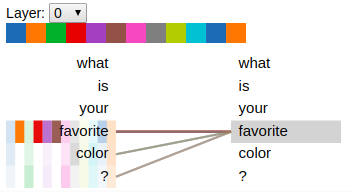
\includegraphics[scale=2]{Figure_4}
		
		
	\end{center}
	\caption[Visualized Attention GPT2]{Visualized Attention GPT2 -- `favorite' shows attention to some but not all words in the sentence.}
	
	
\end{figure}

In our experiments the phrase `What is your favorite color?' is answered with `I love the colors of the rainbow.' This answer does not mention a specific color, as one might expect it should. The diagram might support this observation because `color' on the left is not heavily highlighted. Words like `what' and `your' are barely considered at this head at all. 

%At this layer and at this head, the model does not stress the word `color'. 